
Let
%\label{prob:tri_polar}
\begin{align}
\vec{A} = b\myvec{\cos \theta\\  \sin \theta} ,\vec{B} = \myvec{0\\0},\vec{C} = \myvec{a\\0},
\end{align}
Using the cosine formula, 
\begin{align}
b^2 &= a^2 + c^2 - 2ac \cos B
% \\
% \implies b^2 - c^2 = a^2 - 2ac \cos B &
\\
\implies (b+c)(b-c) &=6^2 - 2(6)\frac{1}{2}c \quad \brak{\because \angle B = 60^{\degree}}
\\
\implies (b+c)(2)&=36-6c \quad \brak{\because b-c = 2}
\\
\text{or, } b+4c &=18
\end{align}
% And we have,
% \begin{align}
% b-c = 2
% \end{align}
From the above, we obtain the matrix equation
\begin{align}
\myvec{1 & 4\\1& -1}\myvec{b\\c} = \myvec{18\\2}
\end{align}
By applying row reduction:
\begin{align}
\myvec{
1 & 4  & 18 
\\
1 & -1   & 2 
}
  \xrightarrow{R_2\rightarrow R_2-R_1}
\myvec{
1 & 4  & 18
\\
0 & -5   & -16 
} 
\\
  \xrightarrow{R_1\rightarrow 5R_1+4R_2} 
\myvec{
5 & 0   & 26 
\\
0 & -5  & -16 
}
\\
 \xrightarrow[R_2 \rightarrow -\frac{R_2}{5}]{R_1\rightarrow \frac{R_1}{5}} 
\myvec{
1 & 0   & \frac{26}{5} 
\\
0 & 1   & \frac{16}{5}
}
\end{align}

\begin{align}
\therefore    \myvec{b\\c}=\myvec{\frac{26}{5}\\\frac{16}{5}}
\end{align}
Thus, the vertices of $\triangle ABC$ are 
\begin{align}
    \vec{A}=\frac{26}{5}\myvec{\cos60\\\sin60}=\myvec{2.6\\4.5} ,\vec{B}=\myvec{0\\0},\vec{C}=\myvec{6\\0}
\end{align}
and the plot of   $\triangle ABC$ is obtained in Fig. \ref{fig:triangle ABC}

\begin{figure}[ht]
    \centering
    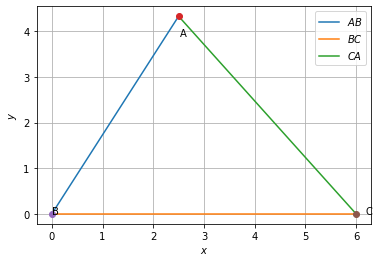
\includegraphics[width=\columnwidth]{solutions/8/fig-1.png}
    \caption{$\triangle ABC$}
    \label{fig:triangle ABC}
\end{figure}






